%\documentclass[format=acmsmall, review=false, screen=true]{acmart}		% ICFP
\documentclass[format=sigplan, review=true]{acmart}		% HASKELL SYMPOSIUM 

\usepackage{float}
\usepackage{graphicx}
\usepackage{subcaption}
\usepackage{ifthen}
\usepackage{minted}
\usepackage{verbatim}

% Metadata Information
%% use defaults for review submission.
\acmConference[HS18]{Haskell Symposium}{2018}{09}
\acmYear{2018}
\copyrightyear{2018}
%\acmDOI{} % \acmDOI{10.1145/nnnnnnn.nnnnnnn}

% Copyright
%% use 'none' for review submission.
\setcopyright{none}
%\setcopyright{acmcopyright}	% = copyright transfer to ACM
%\setcopyright{acmlicensed} 		% = retaining copyright but granting ACM exclusive publication rights
%\setcopyright{rightsretained}  % = open access on payment of a fee
%\setcopyright{usgov}
%\setcopyright{usgovmixed}
%\setcopyright{cagov}
%\setcopyright{cagovmixed}

% TODO : get the data
% DOI
% \acmDOI{0000001.0000001}

% TODO: fill in
% Paper history
\received{March 2018}
%\received[revised]{March 2018}
%\received[accepted]{March 2018}

% Document starts
\begin{document}

% set to true to compile haskell code formated with minted package
% requires pygmentize!
\providecommand\haskellMinted{true}
\ifthenelse{\equal{\haskellMinted}{true} }{
\newminted[HaskellCode]{haskell}{fontsize=\footnotesize}
}{
\newenvironment{HaskellCode}
{\begin{comment}} % seems not to work, don't know why the f***
{\end{comment}}
}

% Title portion. Note the short title for running heads
\title[Functional Pearl: Pure Functional Societies]{Functional Pearl: \\ Purely Functional Societies}
\subtitle{Growing artificial societies: the purely functional way}

\author{Jonathan Thaler}
%\orcid{TODO}
\email{jonathan.thaler@nottingham.ac.uk}
\affiliation{%
  \institution{University of Nottingham}
  \streetaddress{7301 Wollaton Rd}
  \city{Nottingham}
  \postcode{NG8 1BB}
  \country{United Kingdom}}

\begin{abstract}
TODO: instead of using the (boring) SIR model, switch to Sugarscape as it is much more fun and much more interesting

Agent-Based Simulation (ABS) is a methodology in which a system is simulated in a bottom-up approach by modelling the micro interactions of its constituting parts, called agents, out of which the global system behaviour emerges.

So far mainly object-oriented techniques and languages have been used in ABS. In this functional pearl we develop an elegant agent-based implementation of the SIR model of epidemiology, which allows to simulate the spreading of an infectious disease through a population, using using Functional Reactive Programming and Monadic Stream Functions.
\end{abstract}

%
% The code below should be generated by the tool at
% http://dl.acm.org/ccs.cfm
% Please copy and paste the code instead of the example below.
%
% TODO needs to be generated
%\begin{CCSXML}
%<ccs2012>
% <concept>
%  <concept_id>10010520.10010553.10010562</concept_id>
%  <concept_desc>Computer systems organization~Embedded systems</concept_desc>
%  <concept_significance>500</concept_significance>
% </concept>
% <concept>
%  <concept_id>10010520.10010575.10010755</concept_id>
%  <concept_desc>Computer systems organization~Redundancy</concept_desc>
%  <concept_significance>300</concept_significance>
% </concept>
% <concept>
%  <concept_id>10010520.10010553.10010554</concept_id>
%  <concept_desc>Computer systems organization~Robotics</concept_desc>
%  <concept_significance>100</concept_significance>
% </concept>
% <concept>
%  <concept_id>10003033.10003083.10003095</concept_id>
%  <concept_desc>Networks~Network reliability</concept_desc>
%  <concept_significance>100</concept_significance>
% </concept>
%</ccs2012>
%\end{CCSXML}
%
%\ccsdesc[500]{Computer systems organization~Embedded systems}
%\ccsdesc[300]{Computer systems organization~Redundancy}
%\ccsdesc{Computer systems organization~Robotics}
%\ccsdesc[100]{Networks~Network reliability}

%
% End generated code
%

\keywords{Functional Reactive Programming, Monadic \\ Stream Functions, Agent-Based Simulation}

\maketitle

\section{Introduction}
There exists a large number of simulation packages which allow the convenient creation of System Dynamics simulations by straight-forward visual diagram creation. One simply creates stocks and flows, connects them, specifies the flow-rates and initial parameters and then runs the model. An example for such a visual diagram creation in the simulation package AnyLogic can be seen in Figure \ref{fig:sir_stockflow_diagram}.

\begin{figure}
	\centering
	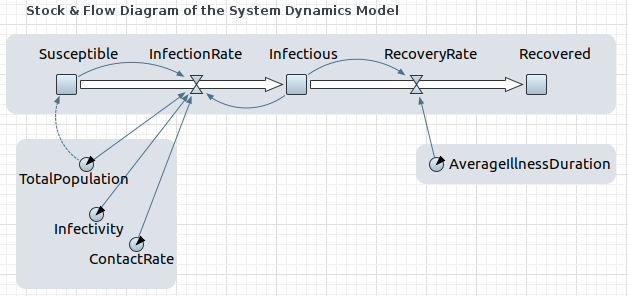
\includegraphics[width=.5\textwidth, angle=0]{./fig/SIR_SD_STOCKFLOW_DIAGRAMM.png}
	\caption{Visual System Dynamics Diagram of the SIR model in AnyLogic Personal Learning Edition 8.3.1.}
	\label{fig:sir_stockflow_diagram}
\end{figure}

Still, implementing System Dynamics directly in code is not as straight forward and involves numerical integration which can be quite tricky to get right. Thus, the aim of this paper is to look into how System Dynamics models can be implemented in code correctly without the use of a simulation package. We use the well known SIR model \cite{kermack_contribution_1927} from epidemiology to demonstrate our approach.

Our language of choice is Haskell because it emphasises a declarative programming style in which one describes \textit{what} instead of \textit{how} to compute. Further it allows to rule out interference with non-deterministic influences or side-effects already at compile-time. This is of fundamental importance for System Dynamics because it behaves completely deterministic and involves no stochastics or non-determinism whatsoever. Also, we make use of Functional Reactive Programming which allows to express continuous-time systems in a functional way. 

We show that by this approach we can arrive at correct-by-construction implementations of System Dynamic models. This means that the correctness of the code is obvious because we have closed the gap between the model specification and its implementation. Thus, the contribution of the paper is the demonstration of how to implement correct-by-construction System Dynamics simulations using Haskell and Functional Reactive Programming.

\subsection{Generalising to Monadic Stream Functions}
\label{sec:generalising_msfs}
A part of the library Dunai is BearRiver, a wrapper which re-implements Yampa on top of Dunai, which should allow us to easily replace Yampa with MSFs. This will enable us to run arbitrary monadic computations in a signal function, solving our problem of correlated random numbers through the use of the Random Monad.

\subsubsection{Identity Monad}
We start by making the transition to BearRiver by simply replacing Yampas signal function by BearRivers', which is the same but takes an additional type parameter \textit{m}, indicating the monadic context. If we replace this type-parameter with the Identity Monad, we should be able to keep the code exactly the same, because BearRiver re-implements all necessary functions we are using from Yampa. We simply re-define the agent signal function, introducing the monad stack our SIR implementation runs in:

\begin{HaskellCode}
type SIRMonad = Identity
type SIRAgent = SF SIRMonad [SIRState] SIRState
\end{HaskellCode}

\subsubsection{Random Monad}
Using the Identity Monad does not gain us anything but it is a first step towards a more general solution. Our next step is to replace the Identity Monad by the Random Monad, which will allow us to run the whole simulation within the Random Monad with the full features of FRP, finally solving the problem of correlated random numbers in an elegant way. We start by re-defining the SIRMonad and SIRAgent:

\begin{HaskellCode}
type SIRMonad g = Rand g
type SIRAgent g = SF (SIRMonad g) [SIRState] SIRState
\end{HaskellCode}

The question is now how to access this Random Monad functionality within the MSF context. For the function \textit{occasionally}, there exists a monadic pendant \textit{occasionallyM} which requires a MonadRandom type-class. Because we are now running within a MonadRandom instance we simply replace \textit{occasionally} with \textit{occasionallyM}. 

\begin{HaskellCode}
occasionallyM :: MonadRandom m => Time -> b -> SF m a (Event b)
-- can be used through the use of arrM and lift
randomBoolM :: RandomGen g => Double -> Rand g Bool
-- this can be used directly as a SF with the arrow notation
drawRandomElemSF :: MonadRandom m => SF m [a] a
\end{HaskellCode}

\subsubsection{Discussion} 
Running in the Random Monad solved the problem of correlated random numbers and elegantly guarantees us that we won't have correlated stochastics as discussed in the previous section. In the next step we introduce the concept of an explicit discrete 2D environment.

\subsection{Adding an environment}
\label{sec:adding_env}
So far we have implicitly assumed a fully connected network amongst agents, where each agent can see and 'knows' every other agent. This is a valid environment and in accordance with the System Dynamics inspired implementation of the SIR model but does not show the real advantage of ABS to situate agents within arbitrary environments. Often, agents are situated within a discrete 2D environment \cite{epstein_growing_1996} which is simply a finite $N x M$ grid with either a Moore or von Neumann neighbourhood (Figure \ref{fig:abs_neighbourhoods}). Agents are either static or can move freely around with cells allowing either single or multiple occupants.

We can directly map the SIR model to a discrete 2D environment by placing the agents on a corresponding 2D grid with an unrestricted neighbourhood. The behaviour of the agents is the same but they select their interactions directly from the shared read-only environment, which will be passed to the agents as input. This allows agents to read the states of all their neighbours which tells them if a neighbour is infected or not. To show the benefit over the System Dynamics approach  and for purposes of a more interesting approach, we restrict the neighbourhood to Moore (Figure \ref{fig:moore_neighbourhood}).

\begin{figure}
\begin{center}
	\begin{tabular}{c c}
		\begin{subfigure}[b]{0.2\textwidth}
			\centering
			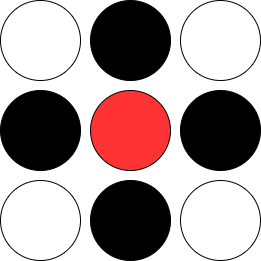
\includegraphics[width=0.5\textwidth, angle=0]{./fig/diagrams/neumann.png}
			\caption{von Neumann}
			\label{fig:neumann_neighbourhood}
		\end{subfigure}
    	&
		\begin{subfigure}[b]{0.2\textwidth}
			\centering
			
\includegraphics[width=0.5\textwidth, angle=0]{./fig/diagrams/moore.png}
			\caption{Moore}
			\label{fig:moore_neighbourhood}
		\end{subfigure}
    \end{tabular}
	\caption{Common neighbourhoods in discrete 2D environments of Agent-Based Simulation.}
	\label{fig:abs_neighbourhoods}
\end{center}
\end{figure}

We also implemented this spatial approach in Java using the well known ABS library RePast \cite{north_complex_2013}, to have a comparison with a state of the art approach and came to the same results as shown in Figure \ref{fig:sir_dunai}. This supports, that our pure functional approach can produce such results as well and compares positively to the state of the art in the ABS field.

\subsubsection{Implementation}
We start by defining the discrete 2D environment for which we use an indexed two dimensional array. Each cell stores the agent state of the last time-step, thus we use the \textit{SIRState} as type for our array data. Also, we re-define the agent signal function to take the structured environment \textit{SIREnv} as input instead of the list of all agents as in our previous approach. As output we keep the \textit{SIRState}, which is the state the agent is currently in. Also we run in the Random Monad as introduced before to avoid the random number correlation. 

\begin{HaskellCode}
type Disc2dCoord = (Int, Int)
type SIREnv      = Array Disc2dCoord SIRState

type SIRAgent g  = SF (Rand g) SIREnv SIRState
\end{HaskellCode}

Note that the environment is not returned as output because the agents do not directly manipulate the environment but only read from it. Again, this enforces the semantics of the \textit{parallel} update-strategy through the types where the agents can only see the previous state of the environment and see the actions of other agents reflected in the environment only in the next step.

Note that we could have chosen to use a StateT transformer with the \textit{SIREnv} as state, instead of passing it as input, with the agents then able to arbitrarily read/write, but this would have violated the semantics of our model because actions of agents would have become visible within the same time-step.

The implementation of the susceptible, infected and recovered agents are almost the same with only the neighbour querying now slightly different. 

Stepping the simulation needs a new approach because in each step we need to collect the agent outputs and update the environment for the next next step. For this we implemented a separate MSF, which receives the coordinates for every agent to be able to update the state in the environment after the agent was run. Note that we need use \textit{mapM} to run the agents because we are running now in the context of the Random Monad. This has the consequence that the agents are in fact run sequentially one after the other but because they cannot see the other agents actions nor observe changes in the shared read-only environment, it is \textit{conceptually} a \textit{parallel} update-strategy where agents run in lock-step, isolated from each other at conceptually the same time.
  
\begin{HaskellCode}
simulationStep :: RandomGen g => [(SIRAgent g, Disc2dCoord)]
               -> SIREnv -> SF (Rand g) () SIREnv
simulationStep sfsCoords env = MSF (\_ -> do
  let (sfs, coords) = unzip sfsCoords 
  -- run agents sequentially but with shared, read-only environment
  ret <- mapM (`unMSF` env) sfs
  -- construct new environment from all agent outputs for next step
  let (as, sfs') = unzip ret
      env' = foldr (\ (a, coord) envAcc -> updateCell coord a envAcc) 
               env (zip as coords)

      sfsCoords' = zip sfs' coords
      cont       = simulationStep sfsCoords' env'
  return (env', cont))
 
updateCell :: Disc2dCoord -> SIRState -> SIREnv -> SIREnv
\end{HaskellCode}

\subsubsection{Results}
We implemented rendering of the environments using the gloss library which allows us to cycle arbitrarily through the steps and inspect the spreading of the disease over time visually as seen in Figure \ref{fig:sir_dunai}.

\begin{figure}
\begin{center}
	\begin{tabular}{c c}
		\begin{subfigure}[b]{0.2\textwidth}
			\centering
			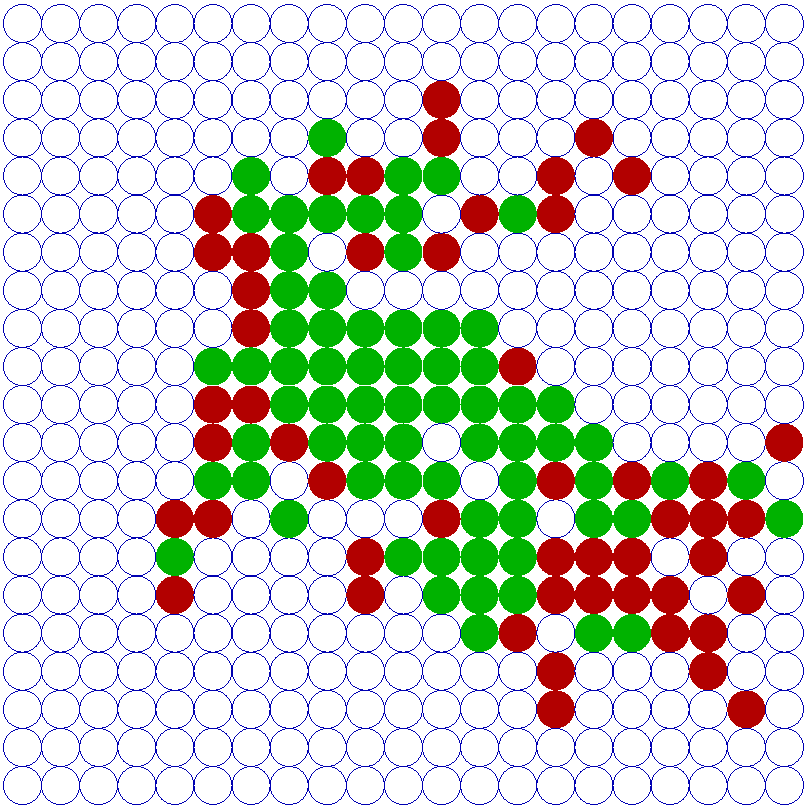
\includegraphics[width=1\textwidth, angle=0]{./fig/SIR_Dunai/SIR_Dunai_dt001_environment.png}
			\caption{Environment at $t = 50$}
			\label{fig:sir_dunai_env}
		\end{subfigure}
    	
    	&
  
		\begin{subfigure}[b]{0.23\textwidth}
			\centering
			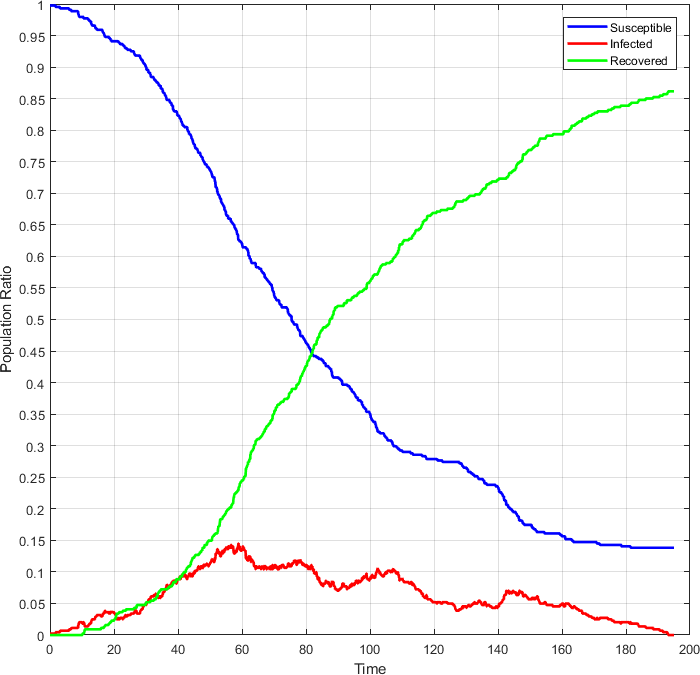
\includegraphics[width=1\textwidth, angle=0]{./fig/SIR_Dunai/SIR_Dunai_dt001.png}
			\caption{Dynamics over time}
			\label{fig:sir_dunai_env_dynamics}
		\end{subfigure}
	\end{tabular}
	
	\caption{Simulating the agent-based SIR model on a 21x21 2D grid with Moore neighbourhood (Figure \ref{fig:moore_neighbourhood}), a single infected agent at the center and same SIR parameters as in Figure \ref{fig:sir_sd_dynamics}. Simulation run until $t = 200$ with fixed $\Delta t = 0.01$. Last infected agent recovers around $t = 194$. The susceptible agents are rendered as blue hollow circles for better contrast.}
	\label{fig:sir_dunai}
\end{center}
\end{figure}

Note that the dynamics of the spatial SIR simulation which are seen in Figure \ref{fig:sir_dunai_env_dynamics} look quite different from the reference dynamics of Figure \ref{fig:sir_sd_dynamics}. This is due to a much more restricted neighbourhood which results in far fewer infected agents at a time and a lower number of recovered agents at the end of the epidemic, meaning that fewer agents got infected overall.

\subsubsection{Discussion}
By introducing a structured environment with a Moore neighbourhood, we showed the ABS ability to place the heterogeneous agents in a generic environment, which is the fundamental advantage of an agent-based approach over other simulation methodologies and allows us to simulate much more realistic scenarios.

Note, that an environment is not restricted to be a discrete 2D grid and can be anything from a continuous N-dimensional space to a complex network - one only needs to change the type of the environment and agent input and provide corresponding neighbourhood querying functions. 

\section{Conclusion and further research}

So far we only looked at recursive simulation in a simulation with a strictly sequential update-strategy where agents are updated in sequence after each other as defined in TODO: cite my Art-Of-Iteration Paper. We leave the question of how Meta-ABS would apply to the parallel update-strategy and whether it is reasonable to extend it to that strategy or not for further research.

Research Questions
\begin{enumerate}
	\item How does deep regression influence the dynamics of a system? Hypothesis: TODO
	\item How do the dynamics of a system change when using perfect information or learning local information? Hypothesis: TODO
	\item Is a hidden markov model suitable for the local learning? Hypothesis: TODO
	\item How can MetaABS best be implemented? Hypothesis: implementing a MetaABS EDSL in a pure functional language like Haskell, should be best suited due to its inherent recursive, declarative nature, which should allow a direct mapping of features of this paradigm to the specification of the meta-model
\end{enumerate}

Problems
\begin{itemize}
	\item Definition of a recursive, declarative description of the Model.
	\item Perfect information about other agents is not realistic and runs counter to agent-based simulation (especially in social sciences) thus an Agent needs to be able to have local, noisy representations of the other agents.
	\item Local representation of other agents could be captured by Hidden Markov Models: observe what other agents do but have hidden interpretation of their internal state - these internal state-representations can be different between the local and the global version whereas the agent learns to represent the global version as best as possible locally.
	\item Infinite regress is theoretically possible but not on computers, we need to terminate at some point
\end{itemize}

\begin{acks}
The authors would like to thank I. Perez, H. Nilsson, J. Greensmith, M. Baerenz, H. Vollbrecht, S. Venkatesan and J. Hey and the referees of Haskell Symposium 2018 for constructive feedback, comments and valuable discussions.
\end{acks}

% Bibliography
\bibliographystyle{ACM-Reference-Format}
%% Citation style
%% Note: author/year citations are required for papers published as an
%% issue of PACMPL.
%%\citestyle{acmauthoryear}   %% For author/year citations
\bibliography{../../../references/phdReferences.bib}

%\begin{appendix}
%\section{Emulating System Dynamics}
The introduction of data-flows in section \ref{sec:step3_dataflow} allows us to emulate the system dynamics (SD) approach because we can now express a system with parallel continuous-time flows between the stocks and flows. Each stock $S(t)$, $I(t)$, $R(t)$ and each flow $infectionRate$, $recoveryRate$ is implemented as an agent with a fixed agent id. The connections between them are implemented using the previously introduced data-flow mechanism. We start by refining the types for our SIR implementation:

\begin{minted}[fontsize=\footnotesize]{haskell}
type SDMsg      = Double
type SDAgentIn  = AgentIn SDMsg
type SDObs      = Maybe Double
type SDEntity   = Agent SDObs SDMsg
type SDEntityId = AgentId

totalPopulation :: Double
totalPopulation = 1000

infectedCount :: Double
infectedCount = 1
\end{minted}

The message-data is now a plain Double and the observable data has been changed to a \textit{Maybe} Double: instead of discrete agent-states we are dealing now with stocks and flows which are aggregates represented by continuous values. Note that we use a Maybe type as flows only connect stocks and transform their values but don't have any observable state themselves. Note also that the population size and number of infected is specified now as Double as we are dealing with continuous aggregates.

We give hard-coded agent ids to our stocks and flows. This allows then for setting up hard-coded connections between them at compile time.
\begin{minted}[fontsize=\footnotesize]{haskell}
susceptibleStockId :: SDEntityId
susceptibleStockId = 0

infectiousStockId :: SDEntityId
infectiousStockId = 1

recoveredStockId :: SDEntityId
recoveredStockId = 2

infectionRateFlowId :: SDEntityId
infectionRateFlowId = 3

recoveryRateFlowId :: SDEntityId
recoveryRateFlowId = 4
\end{minted}

Next we give the implementation of the infectious stock (the implementations of the susceptible and recovered stock work in a similar way and are left as an easy exercise to the reader):

\begin{minted}[fontsize=\footnotesize]{haskell}
infectiousStock :: Double -> SDEntity
infectiousStock initValue = proc ain -> do
  let infectionRate = flowInFrom infectionRateFlowId ain
      recoveryRate  = flowInFrom recoveryRateFlowId ain

  stockValue <- (initValue+) ^<< integral -< (infectionRate - recoveryRate)
  
  let ao   = agentOut (Just stockValue)
      ao'  = dataFlow (infectionRateFlowId, stockValue) ao
      ao'' = dataFlow (recoveryRateFlowId, stockValue) ao'
      
  returnA -< ao''
\end{minted}

The stock receives flows from both the infection-rate and recovery-rate flow using the function \textit{flowInFrom} (see below). Then the current stock value is calculated using the \textit{integral} function of Yampa with an initial value added which are the initially infected people. The integral primitive of Yampa integrates the fed in data over time using the rectangle rule which means it simply multiplies the input values by the current $\Delta t$ and accumulates them. Note that we can directly express the SD equation using Yampas DSL for continuous-time systems. The current stock value is then set as the observable value of the stock and sent to the infection- and recovery-rate flows. For convenience we implemented an additional function \textit{flowInFrom} which returns the first value sent from the corresponding agent id or 0.0 if none was sent.

\begin{minted}[fontsize=\footnotesize]{haskell}
flowInFrom :: SDEntityId -> SDAgentIn -> Double
flowInFrom senderId ain = firstValue dsFiltered
  where 
    dsFiltered = filter ((==senderId) . fst) (aiData ain)

    firstValue :: [AgentData SDMsg] -> Double
    firstValue [] = 0.0
    firstValue ((_, v) : _) = v
\end{minted}
	
The \textit{infectionRate} flow is implemented as follows (the implementations of the recovery-rate flow works in a similar way and is left as an easy exercise to the reader):

\begin{minted}[fontsize=\footnotesize]{haskell}
infectionRateFlow :: SDEntity
infectionRateFlow = proc ain -> do
  let susceptible = flowInFrom susceptibleStockId ain 
      infectious  = flowInFrom infectiousStockId ain

      flowValue   = (infectious * contactRate * susceptible * infectivity) / totalPopulation
  
      ao          = agentOut Nothing
      ao'         = dataFlow (susceptibleStockId, flowValue) ao
      ao''        = dataFlow (infectiousStockId, flowValue) ao'
      
  returnA -< ao''
\end{minted}

Instead of integrating a value over time a stock just transforms incoming values from the connected stocks - in this case the susceptible and infectious stocks. Note again how directly we can express the formula for the infection rate.

When running the simulation one must make sure to use a small enough $\Delta t$ as \textit{integral} of Yampa is implemented using the rectangle rule which leads to considerable numerical errors with large $\Delta t$. Figure \ref{fig:sir_sd_dynamics} was created with this SD emulation for which we used $\Delta t = 0.01$.
%
%\subsection{Step VI: Adding agent transactions}
Imagine two agents A and B want to engage in a bartering process where agent A, is the seller who wants to sell an asset to agent B who is the buyer. Agent A sends Agent B a sell offer depending on how much agent A values this asset. Agent B receives this sell offer, checks if the price satisfies its utility, if it has enough wealth to buy the asset and replies with either a refusal or its own price offer. Agent A then considers agent Bs offer and if it is happy it replies to agent B with an acceptance of the offer, removes the asset from its inventory and increases its wealth. Agent B receives this acceptance offer, puts the asset in its inventory and decreases its wealth (note that this process could involve a potentially arbitrary number of steps without loss of generality).
We can see this behaviour as a kind of multi-step transactional behaviour because agents have to respect their budget constraints which means that they cannot spend more wealth or assets than they have. This implies that they have to 'lock' the asset and the amount of cash they are bartering about during the bartering process. If both come to an agreement they will swap the asset and the cash and if they refuse their offers they have to 'unlock' them.
In classic OO implementations it is quite easy to implement this as normally only one agent is active at a time due to sequential (discrete event scheduling approach) scheduling of the simulation. This allows then agent A which is active, to directly interact with agent B through method calls. The sequential updating ensures that no other agent will touch the asset or cash and the direct method calls ensure a synchronous updating of the mutable state of both objects with no time passing between these updates.
TODO: this is a novel concept as it is implicitly there already in OO implementations due to global mutual state.

TX: running agents and with 0 dt is easy with bearriver.
%\end{appendix}

\end{document}
